% DOCUMENT FORMAT ======================= -*- mode: LaTeX; coding: utf-8 -*- ===

\documentclass[diploma]{softlab-thesis}


% PACKAGE SETTINGS =============================================================

\usepackage{fontspec}
\usepackage{amsmath}
\usepackage{amsfonts}
\usepackage{multirow}
\usepackage{array}
\usepackage{mdwlist}
\usepackage{subfig}
\usepackage{floatrow}
\usepackage{float}
\usepackage{verbatim}
\usepackage{color}
\usepackage{graphicx}
\usepackage{xunicode}
\usepackage{xltxtra}
\usepackage{url}
%\usepackage{dsfont}
%\usepackage{microtype}
\usepackage{hyphenat}
\usepackage{multicol}
\usepackage{wrapfig}
\usepackage{lipsum}
\usepackage{listings}
\usepackage{paralist}
\usepackage{ulem}
\usepackage{tocvsec2}
\usepackage{url}
\usepackage[toc,page]{appendix}
% FONT SETTINGS ===============================================================

%\setromanfont[Mapping=tex-text]{CMU Serif}
%%\setromanfont[Mapping=tex-text]{CMU Sans Serif} % temporary change until printing
%%\setsansfont[Mapping=tex-text]{CMU Sans Serif}
%%\setmonofont[Mapping=tex-text]{CMU Typewriter Text}
%\setmainfont[Mapping=tex-text]{CMU Serif}
%%\setmainfont[Mapping=tex-text]{CMU Sans Serif}  % temporary change until printing

%\setromanfont[Mapping=tex-text,ExternalLocation=fonts/]{cmunrm.otf}
%\setsansfont[Mapping=tex-text,ExternalLocation=fonts/]{cmunss.otf}
%\setmonofont[Mapping=tex-text,ExternalLocation=fonts/]{cmuntt.otf}
%\setmainfont[Mapping=tex-text, ExternalLocation=fonts/]{cmunss.otf}

\defaultfontfeatures{Mapping=tex-text}
%\setromanfont{Linux Libertine O}
\setromanfont{DroidSerif}

% CUSTOM COLORS ===============================================================

\definecolor{gray}{rgb}{0.5,0.5,0.5}
\definecolor{darkgreen}{rgb}{0.0,0.5,0.0}
\definecolor{mygreen}{rgb}{0,0.6,0}
\definecolor{mygray}{rgb}{0.5,0.5,0.5}
\definecolor{mymauve}{rgb}{0.58,0,0.82}
\definecolor{myorange}{RGB}{246,177,50}

% CUSTOM COMMANDS =============================================================

\newcommand\fixme{\textrm{\textbf{\textcolor{red}{FIXME: }}}}
\newcommand\todo{\textrm{\textbf{\textcolor{myorange}{TODO: }}}}
\newcommand\mytilde{\raise.17ex\hbox{$\scriptstyle\sim$}}
\newcommand\okeanos{\textbf{\raise.17ex\hbox{$\scriptstyle\sim$}okeanos }}


% Layout macros
\newcommand\spa[1]{\; #1 \;}

% Font macros
\newcommand\resfont[1]{\ensuremath{\mathtt{#1}}}

% Mathematical macros
\newcommand\setmap[3]{#1\{#2 \mapsto #3\}}
\newcommand\getmap[3]{(#2 \mapsto #3) \in #1}
\newcommand\tuple[2]{\ensuremath{\langle#1, #2\rangle}}
\newcommand\mfrac[2]{\ensuremath{\dfrac{#1}{#2}}}
\newcommand\nequiv[2]{\ensuremath{#1 \not\equiv #2}}

% Core Ruby Operational Semantics letter bindings
\newcommand\mem{\mu}

% Core Ruby Operational Semantics low level macros
\newcommand\state[2]{(#1, #2)}
\newcommand\transition[1]{\ensuremath{\overset{#1, c*}{\rightarrow}}}
\newcommand\range[2]{#1, ..., #2}
\newcommand\midrange[5]{\range{#1}{#2}, #3, \range{#4}{#5}}

% Core Ruby Operational Semantics high level macros
\newcommand\operation[5]{\ensuremath{\state{#1}{#2} \transition{#3} \state{#4}{#5}}}
\newcommand\propagation[2]{\operation{#1}{\mem}{#2}{#1'}{\mem'}}

% Core Ruby specific Operational Semantics macros
\newcommand\semicolon[2]{#1; \; #2}
\newcommand\assign[2]{#1 = #2}
\newcommand\mcall[3]{#1.\texttt{#2}(#3)}
\newcommand\ifte[3]{\resfont{if} \; #1 \; \resfont{then} \; #2 \; \resfont{else} \; #3}
\newcommand\newclass[2]{#1.\resfont{new}(#2)}
\newcommand\methoddef[3]{\resfont{def} \; #1(#2) = #3}
\newcommand\classdef[2]{\resfont{class} \; #1 = #2}
\newcommand\with[3]{with \; \tuple{#1}{#2} \; do \; #3}

% Success Typing macros
\newcommand\ssub{\sqsubseteq\_S}

% Core Ruby Success Typing letter bindings
\newcommand\classlist{\Delta}
\newcommand\envir{\Gamma}
\newcommand\fields{\Phi}
\newcommand\currclass{l}

% Core Ruby Success Typing inferencing macros
\newcommand\stinfer[5]{\classlist; \; #1; \; \fields \; \underset{\currclass}{\vdash} \; #2: #3 \; \& \; #4; \; #5}


%%%%%%%%%%%%%%%%%%%%%%%%%%% CACHED STUFF %%%%%%%%%%%%%%%%%%%%%%%%%%%

\newcommand\xcache{\texttt{xcache} }

%%%%%%%%%%%%%%%%%%%%%%%%%%% HASKELL STUFF %%%%%%%%%%%%%%%%%%%%%%%%%%%

%\newcommand\typerep[1]{\ensuremath{#1}}
\newcommand\typerep[1]{\lstinline[basicstyle=\normalsize\ttfamily,keywords={}]|#1|}
\newcommand\typefootrep[1]{\textbf{\lstinline[basicstyle=\footnotesize\ttfamily,keywords={}]|#1|}}
% \newcommand\ttyperep[1]{\typerep{#1}}
% \newcommand\mtyperep[1]{\mbox{\typerep{#1}}}

% Arrow types
\newcommand\typeto[2]{\typerep{#1} \typerep{->} \typerep{#2}}
\newcommand\typetotwo[3]{\ensuremath{\typerep{#1} \typerep{->}
                                     \typerep{#2} \typerep{->}
                                     \typerep{#3}}}

\newcommand\tyconapone[2]{\ensuremath{\mbox{\typerep{#1}} \:\: \mbox{#2}}}
\newcommand\tyconaponeC[2]{\ensuremath{\mbox{\typerep{#1}} \:\: \mbox{\typerep{#2}}}}
% \newcommand\tyconapone[2]{\typerep{#1} $\:$ \typerep{#2}}

\newcommand\tyconaptwo[3]{\ensuremath{\mbox{\typerep{#1}} \:\: \mbox{#2} \:\: \mbox{#3}}}


% FIGURE SETUP ===============================================================

\newcommand\diagram[2]{
	\begin{figure}[h!]
		\centering
		\includegraphics[width=\textwidth,height=\textheight,keepaspectratio]
		{diagrams/#2}
		\caption{#1}
		\label{fig:#2}
	\end{figure}
}

\newcommand\diagramscale[3]{
	\begin{figure}[h!]
		\centering
		\includegraphics[scale={#3}]
		{diagrams/#2}
		\caption{#1}
		\label{fig:#2}
	\end{figure}
}
\newcommand\diagramstrict[2]{
	\begin{figure}[H]
		\centering
		\includegraphics[keepaspectratio]
		{diagrams/#2}
		\caption{#1}
		\label{fig:#2}
	\end{figure}
}


% SPELLING =====================================================================

% CODE HIGHLIGHTING ============================================================

% Define common settings for code listings

\lstset{
	backgroundcolor=\color{white},
	basicstyle=\small\ttfamily,		% style for code
	breakatwhitespace=false,        % sets if automatic breaks should only
									% happen at whitespace
	breaklines=true,                % sets automatic line breaking
	captionpos=b,                   % sets the caption-position to bottom
	commentstyle=\color{mygreen},   % style for comments
	escapeinside={\%*}{*)},         % if you want to add LaTeX within your code
	frame=single,                   % adds a frame around the code
	keepspaces=true,                % keeps spaces in text, useful for
	%keywordstyle=\color{blue}\bfseries,
					% keyword style
	numbers=left,
	numbersep=5pt,                  % how far the line-numbers are from the
					% code
	numberstyle=\tiny\color{mygray},% style for line-numbers
	rulecolor=\color{black},
	stepnumber=1,                   % the step between two line-numbers. If
					% it's 1, each line will be numbered
	stringstyle=\color{mymauve},    % style for strings
	tabsize=2,                      % sets default tabsize to 2 spaces
}

% Define specific rules for each language

\lstdefinestyle{c}
{
	language=C,
	tabsize=4
}

\lstdefinestyle{haskell}
{
	language=Haskell
}

\lstdefinestyle{ruby}
{
	language=Ruby
}

\lstdefinestyle{erlang}
{
	language=Erlang.
	captionpos=
}

\lstdefinestyle{plain}
{
	stepnumber=0
}

% Create new commands for simpler usage

\newcommand\ccode[2]{
	\lstinputlisting[float=h!, style=c, caption={#1}, label=lst:#2]{src/#2}
}

\newcommand\pcode[2]{
	\lstinputlisting[float=h!, language=Python, caption={#1},label=lst:#2]{src/#2}
}

\newcommand\bcode[2]{
	\lstinputlisting[float=h!, language=bash, caption={#1},label=lst:#2]{src/#2}
}
\newcommand\cccode[2]{
	\lstinputlisting[style=c, caption={#1}, label=lst:#2]{src/#2}
}

\newcommand\haskellcode[3]{
	\lstinputlisting[style=haskell, caption={#1}, label=lst:#2]{src/#3}
}

\newcommand\rubycode[2]{
	\lstinputlisting[style=ruby, caption={#1}, label=lst:#1]{src/#2}
}

\newcommand\erlangcode[2]{
	\lstinputlisting[style=erlang, caption={#1}, label=lst:#1]{src/#1}
}

\newcommand\plaintext[2]{
	\lstinputlisting[float=h!, style=plain, caption={#1},
	label=lst:#2]{src/#2}
}

% CHANGE MATH FONT ============================================================

% HYPERREF MUST BE LAST =======================================================

\usepackage[xetex,colorlinks=true,linkcolor=blue,citecolor=darkgreen]{hyperref}

% DOCUMENT INFORMATION =========================================================

\title{Probabilistic attacks against compressed encrypted protocols}

% ===============> FIXME
\author{Δημήτριος Καρακώστας}
\authoren{Dimitrios Karakostas}
\datedefense{0}{0}{0}
\supervisor{FIXME}
\supervisorpos{FIXME}
\committeeone{FIXME}
\committeeonepos{FIXME}
\committeetwo{FIXME}
\committeetwopos{FIXME}
\committeethree{FIXME}
\committeethreepos{FIXME}
\hypersetup{
	pdftitle={},
	pdfauthor={test},
	pdfsubject={},
	pdfkeywords={}
}


% MAIN DOCUMENT ================================================================

\begin{document}

\frontmatter
%\maketitle

\def\templen{\parindent}
\setlength{\parindent}{0pt}
\setlength{\parskip}{1.5ex plus 0.5ex minus 0.2ex}
%\begin{abstractgr}

Η ασφάλεια είναι ένα από τα βασικά χαρακτηριστικά κάθε σύγχρονου υπολογιστικού
συστήματος. Η παρούσα εργασία ερευνά επιθέσεις πάνω σε συμπιεσμένα
κρυπτογραφημένα πρωτόκολλα.

Συγκεκριμένα, προτείνεται μια νέα ιδιότητα που χαρακτηρίζει κρυπτοσυστήματα, η
μη-διακρισιμότητα ενάντια σε επιθέσεις μερικώς επιλεγμένου κειμένου (IND-PCPA),
καθώς και ένα μοντέλο επίθεσης που χρησιμοποιεί αυτή την ιδιότητα. Προκειμένου
να ξεπεραστούν εμπόδια που παρουσιάζονται σε συστήματα του πραγματικού κόσμου,
προτείνονται στατιστικές μέθοδοι, οι οποίες βελτιώνουν την επίδοση και
εγκυρότητα της επίθεσης.

Τα πειράματα που διεξήχθησαν κατά τη διάρκεια της εργασίας αφορούσαν σε δύο
ευρέως χρησιμοποιούμενα συστήματα, το Facebook Chat και το Gmail, για την
επίτευξη των οποίων χρησιμοποιήθηκε λογισμικό, το οποίο αναπτύχθηκε σε Python
για τους σκοπούς αυτής της εργασίας. Τα πειράματα έγιναν σε συνθήκες εργαστηρίου
και απέδειξαν ότι τα δύο αυτά συστήματα δεν είναι IND-PCPA, όσον αφορά
συγκεκριμένους τύπους μυστικών.

Τέλος, προτείνονται καινοτόμες τεχνικές, οι οποίες θα οδηγήσουν σε πλήρη
αντιμετώπιση επιθέσεων που ακολουθούν το μοντέλο που προτείνεται, όπως η
επίθεση που παρουσιάστηκε στην παρούσα εργασία.

\end{abstractgr}

\begin{abstracten}

Security is a fundamental aspect of every modern system. This work investigates
attacks on compressed encrypted protocols.

A new property of cryptosystems is proposed, cited Indistinguishability under
Partially Chosen Plaintext Attack (IND-PCPA), along with an attack model that
works under such a mechanism. In order to bypass obstacles of real-world
systems, statistical methods were proposed, to improve the performance and
validity of the attack.

Experiments were conducted on two widely used systems, Facebook Chat and Gmail, using
a Python framework, that was implemented for the purpose of this paper. Results
in lab environment revealed that those two systems are not IND-PCPA, regarding
certain specified types of secrets.

Finally, novel techniques were proposed, that could lead to complete mitigation
of attacks that follow the proposed model.

\end{abstracten}


\setlength{\parindent}{\templen}
\setlength{\parskip}{0pt}
\tableofcontents
%\listoffigures
%\listoftables
%\renewcommand{\lstlistlistingname}{List of Listings}
%\lstlistoflistings % changed the title above

\mainmatter
% moved these two commands here so that they don't influence the toc
\setlength{\parindent}{0pt}
\setlength{\parskip}{1.5ex plus 0.5ex minus 0.2ex}

\renewcommand\floatpagefraction{.7}

%\chapter{Εισαγωγή}\label{ch:intro}
\epigraph{\itshape Even if you're not doing anything wrong, you are being watched and
recorded.}{---Edward Snowden}

\section{Εισαγωγή}\label{sec:intro}

Το καλοκαίρι του 2013 επιβεβαιώθηκε αυτό που υπήρχε ως υποψία όλα τα προηγούμενα
χρόνια: οι συνομιλίες παρακολουθούνται και τα δεδομένα που ανταλλάσσονται μέσω
Διαδικτύου δεν είναι ασφαλή. Οι αποκαλύψεις Snowden άλλαξαν τον τρόπο με τον
οποίο αντιλαμβανόμαστε τη χρήση online υπηρεσιών και έστρεψαν πολλούς ερευνητές
και χρήστες στην αναζήτηση λύσεων ώστε οι επικοινωνίες να γίνουν πιο ασφαλείς
απέναντι σε κάθε είδους αντιπάλους.

Η παρούσα εργασία στοχεύει να αναδείξει αδυναμίες στα πρωτόκολλα που επιτρέπουν
την επικοινωνία μέσω Διαδικτύου και μέσω της δημοσίευσής της να κινητοποιήσει
την κοινότητα ώστε να αντιμετωπιστούν αυτά τα προβλήματα.

Η έρευνά μας επικεντρώνεται σε επιθέσεις που εκμεταλλεύονται τους αλγόριθμους
συμπίεσης που χρησιμοποιούνται πάνω στα δεδομένα που ανταλλάσσονται, προτού αυτά
κρυπτογραφηθούν και αποσταλούν. Συγκεκριμένα, επεκτείνουμε υπάρχοντα μο-ντέλα,
όπως το BREACH, ώστε να καταδείξουμε πως πρωτόκολλα τα οποία θεωρούνται σήμερα
απολύτως ασφαλή είναι πρακτικά τρωτά σε παρόμοιες επιθέσεις.

Κατά τη διάρκεια της έρευνάς μας επικεντρωθήκαμε στο λογισμικό συμπίεσης gzip,
το οποίο εφαρμόζει τον αλγόριθμο DEFLATE, ο οποίος με τη σειρά του αποτελεί
συνδυασμό των αλγορίθμων συμπίεσης Huffman και LZ77. Συγκεκριμένα, η επίθεση
εκμεταλλεύε-ται την ανάλυση που κάνει ο LZ77 πάνω στο καθαρό κείμενο, ενώ
αντίθετα η ύπαρξη συμπίεσης Huffman εμποδίζει την εκτέλεση. Παρότι δεν ελέγξαμε
άλλους αλγόριθμους ή εμπορικές εφαρμογές συμπίεσης, είναι αρκετά ασφαλές να
υποθέσουμε πως αλγόριθ-μοι που ακολουθούν όμοιες τεχνικές είναι δυνητικά στόχοι
για παρόμοιες επιθέσεις.

Το πιο διαδεδομένο πρωτόκολλο ανταλλαγής δεδομένων στο Διαδίκτυο είναι το HTTP
(Hyper-Text Transfer Protocol). Είναι ευρέως αποδεκτό πως δεδομένα που
στέλνονται μέσω απλού HTTP και δεν είναι κρυπτογραφημένα θα πρέπει να
θεωρούνται ανασφαλή ως προς την ακεραιότητα και την αυθεντικότητά τους. Το κενό
στην ασφάλεια που αφήνει το απλό HTTP ήρθε να συμπληρώσει αρχικά το SSL (Secure
Socket Layer) και στη συνέχεια το TLS (Transport Layer Security). Το TLS
εισάγεται ως ένα επίπεδο δικτύου πριν το επίπεδο εφαρμογής και επιβάλλει την
κρυπτογράφηση των δεδομένων πριν αυτά σταλούν στο Διαδίκτυο.

Οι αλγόριθμοι κρυπτογράφησης που χρησιμοποιούνται εν γένει μπορούν να χωριστούν
σε δύο κύριες κατηγορίες: ροής και δέσμης. Στην πρώτη περίπτωση, τα δεδομένα
κρυ-πτογραφούνται ως μια συνεχής ροή, ενώ στη δεύτερη περίπτωση χωρίζονται σε
δέσμες ίσου μεγέθους και κρυπτογραφείται κάθε δέσμη χωριστά. Σε περίπτωση που τα
δεδομέ-να δεν κατανέμονται με ακρίβεια σε δέσμες, εισάγεται τεχνητός θόρυβος
ώστε να επιτευχθεί το επιθυμητό μέγεθος.

Ο κυριότερος αλγόριθμος ροής είναι ο RC4, ο οποίος πλέον θεωρείται ανασφαλής και
αποφεύγεται η χρήση του. Από την άλλη πλευρά, ο πιο διαδεδομένος αλγόριθμος
δέσμης είναι ο AES, ο οποίος χρησιμοποιείται σε διάφορες παραλλαγές από την
πλειοψηφία των συστημάτων. Η χρήση αλγορίθμων ροής καθιστά την επίθεση που
περιγράφουμε πολύ ευκολότερη, καθώς μειώνεται η ύπαρξη θορύβου που μπορεί να
επηρεάσει τα αποτελέσματα. Ωστόσο, κατά τη διάρκεια της έρευνάς μας, διαπιστώσαμε πως η
χρήση του AES δεν εξασφαλίζει απόλυτη ασφάλεια και υπό προϋποθέσεις είναι δυνατό
δεδομέ-να που ανταλλάσσονται με αυτές τις μεθόδους να υποκλαπούν.

Για να το επιτύχουμε αυτό έπρεπε αρχικά να μοντελοποιήσουμε την επίθεσή μας. Για
το σκοπό αυτό ορίσαμε μια νέα κρυπτογραφική ιδιότητα, την οποία ονομάζουμε
μη-διακρισιμότητα ενάντια σε επιθέσεις μερικώς επιλεγμένου κειμένου (IND-PCPA). Όμοιες
ιδιότητες, όπως IND-CPA, IND-CCA κ.ά, είναι ορισμένες στη βιβλιογραφία και
χρησιμοποιούνται ευρέως στην ανάλυση κρυπτοσυστημάτων. Η εισαγωγή της IND-PCPA
στοχεύει στην επέκταση των αναλύσεων ώστε να καλύπτουν επιθέσεις όπως αυτή που
αναπτύσσεται στην παρούσα εργασία.

Η επιτυχία της επίθεσης προϋποθέτει το σύστημα το οποίο αναλύεται να παρουσιάζει
συγκεκριμένα χαρακτηριστικά-παθογένειες. Η επίλυση των παθογενειών είναι
δεδομέ-νο πως βοηθάει σε σημαντικό βαθμό στην αντιμετώπιση της επίθεσης. Συνεπώς,
είναι σημαντικό να μοντελοποιήσουμε την επίθεση και να ορίσουμε τα
χαρακτηριστικά της, προτού επιχειρήσουμε να βρούμε τρόπους αντιμετώπισής της.

Η επίθεση που ερευνάται είναι επέκταση γνωστών μοντέλων, όπως αναφέρθηκε. Ωστό-σο
η ανάλυσή μας οδηγεί σε χαλάρωση των απαιτήσεων που θεωρούνταν δεδομένες και,
κατά συνέπεια, στοχεύει σε μεγαλύτερο εύρος συστημάτων. Είναι εμφανές πως
σε οποιοδήποτε σύστημα ικανοποιούνται οι απαιτήσεις που ορίζουμε η επίθεση είναι
δυνητικά εφικτή, συνεπώς το σύστημα θα πρέπει να θεωρείται ανασφαλές.

Στην παρούσα εργασία περιγράφονται αδυναμίες σε δύο εφαρμογές που
χρησιμοποιού-νται από μεγάλο ποσοστό χρηστών του Διαδικτύου. Η πρώτη είναι η
υπηρεσία chat του Facebook, όπου αναλύουμε τον τρόπο με τον οποίο προσωπικά
μηνύματα κάποιου χρήστη μπορούν να υποκλαπούν. Η δεύτερη είναι η υπηρεσία email
της Google, το Gmail. Σε αυτή την περίπτωση, παρουσιάζουμε πώς μπορεί κάποιος
επιτιθέμενος να αποκτήσει τον έλεγχο του λογαριασμού ενός χρήστη ώστε να είναι
σε θέση να υποδυθεί τον χρήστη, καθώς και να υποκλέψει δεδομένα που
ανταλλάχθησαν μέσω mail.

Για την εκτέλεση των πειραμάτων αναπτύξαμε λογισμικό σε επίπεδο
proof-of-concept, το οποίο μπορεί να χρησιμοποιηθεί για την εκτέλεση της
επίθεσης στα συγκεκριμένα συστήματα. Ωστόσο κάθε σύστημα παρουσιάζει
ιδιομορφίες, συνεπώς για να χρησιμο-ποιηθεί το ίδιο λογισμικό για την ανάλυση
άλλων συστημάτων θα πρέπει να προηγηθούν οι κατάλληλες τροποποιήσεις.

Σε αυτό το σημείο είναι σημαντικό να επικεντρωθούμε στο στατιστικό κομμάτι της
επίθεσης. Η επίθεση δεν μπορεί να θεωρηθεί ντετερμινιστική, καθώς η ανάλυσή μας
βασίζεται στη χρήση πιθανοτήτων. Είναι εμφανές ωστόσο πως στο βαθμό που
εξασφα-λίζουμε μεγαλύτερη εμπιστοσύνη και μειώνουμε το στατιστικό λάθος, τα
αποτελέσματα είναι δυνατό να προκύψουν σε λιγότερο χρόνο και με μεγαλύτερη
ακρίβεια.

Ο πιθανοτικός παράγοντας της επίθεσης μας οδήγησε στην ανάπτυξη μεθόδων
βελτι-στοποίησης. Ο στόχος μας αφορά σε δύο κατευθύνσεις: μείωση των στατιστικών
δειγμά-των και ελαχιστοποίηση του χρόνου συλλογής κάθε δείγματος.

Στην πρώτη περίπτωση είναι αναγκαίο να οριστεί ένα κατάλληλο πλήθος δειγμάτων,
τα οποία οδηγούν σε ένα ασφαλές συμπέρασμα. Βάσει του νόμου των μεγάλων αριθμών,
όσο περισσότερα δείγματα συλλέγουμε τόσο καλύτερα αποτελέσματα αναμένουμε.
Ωστόσο από ένα σημείο και μετά ο χρόνος εκτέλεσης καθιστά μεγαλύτερο πλήθος
δειγμάτων απαγορευτικό. Για αυτό το λόγο αναλύσαμε την στατιστική κατανομή του
θορύβου και καταλήξαμε σε συγκεκριμένο πλήθος δειγμάτων από το οποίο μπορούν να
προκύψουν αξιόπιστα αποτελέσματα για κάθε περίπτωση.

Στη δεύτερη περίπτωση ερευνήσαμε τη λειτουργία των προγραμμάτων περιήγησης του
Διαδικτύο (browsers) και των προτοκόλλων των επιπέδων μεταφοράς και δικτύου.
Δημιουργήσαμε τεχνικές παραλληλοποίησης, οι οποίες επιτρέπουν τη διαίρεση των
αναγκαίων δειγμάτων με αποδοτικές μεθόδους και τη συλλογή τους από πολλές πηγές
ταυτόχρονα. Εν τέλει, κάθε τεχνική μπορεί να οδηγήσει σε επιτάχυνση της επίθεσης
κατά αρκετές τάξεις μεγέθους.

Τα αποτελέσματα που προέκυψαν για τις υπηρεσίες που ελέγξαμε μπορούν να
θεωρη-θούν επιτυχημένα. Συγκεκριμένα, αποδείξαμε ότι οι αδυναμίες που βρήκαμε
μπορούν να χρησιμοποιηθούν όπως αναμέναμε και καταφέραμε να υποκλέψουμε
τουλάχιστον ένα byte δεδομένων σε κάθε περίπτωση. Ωστόσο, ο χρόνος που
απαιτείται για την ολοκλήρωση της επίθεσης είναι της τάξης των εβδομάδων ή
μηνών, συνεπώς, ανάλογα με τις απαιτήσεις του επιτιθέμενου, η επίθεση μπορεί να
θεωρηθεί μη-ρεαλιστική. Σε κάθε περίπτωση, τα αποτελέσματά μας καταδεικνύουν ότι
τα συστήματα που αναλύσα-με, στο βαθμό και υπό τις προϋποθέσεις που περιγράψαμε,
θα πρέπει να θεωρούνται ανασφαλή.

Η αντιμετώπιση της επίθεσης θα πρέπει να αποτελέσει αντικείμενο μελέτης και να
υλοποιηθεί το συντομότερο δυνατόν. Η φύση της επίθεσης επιτρέπει επιλεκτικές
λύσεις, οι οποίες βελτιώνουν την ασφάλεια υπό προϋποθέσεις. Ωστόσο είναι
απαραίτητο να υλοποιηθούν πρότυπα τα οποία επικεντρώνονται στα δομικά προβλήματα
που επιτρέ-πουν τέτοιου είδους επιθέσεις και αντιμετωπίζουν ολοκληρωτικά τις
παθογένειες.

Στη βιβλιογραφία μπορούν να βρεθούν πλήθος προτάσεων που ως ένα βαθμό οδηγούν
σε βελτίωση της ασφάλειας των συστημάτων. Στην παρούσα εργασία αναλύουμε αρκε-τές
τέτοιες προτάσεις και εξηγούμε για ποιο λόγο δεν αποτελούν ριζική αντιμετώπιση
του προβλήματος. Στη συνέχεια, παρουσιάζουμε πρότυπα τα οποία εφόσον
υλοποιη-θούν είναι δυνατόν να εξαλείψουν ολοκληρωτικά επιθέσεις όπως αυτή που
ερευνήσαμε.

Εν τέλει, η παρούσα εργασία αποτελεί τη συνέχεια μια ομάδας ερευνών που
παρουσιά-στηκαν τα τελευταία χρόνια και φανέρωσαν βασικές αδυναμίες στα
συστήματα που χρησιμοποιούμε κατά κόρον. Είναι σημαντικό να επεκταθεί με νέες
τεχνικές βελτιστο-ποίησης της επίθεσης και, κυρίως, νέες μεθόδους αντιμετώπισής
της.

\section{Δομή της εργασίας}\label{sec:structure}

Η εργασία έχει δομηθεί ως εξής:

\begin{description} \item{Κεφάλαιο \ref{background}} \hfill \\

Το κεφάλαιο αυτό παρέχει στον αναγνώστη βασικές πληροφορίες, τόσο σε τεχνικό όσο
και σε θεωρητικό επίπεδο, οι οποίες θα χρησιμοποιηθούν στη συνέχεια.
Θα περιγράψουμε τους πιο διαδεδομένους αλγόριθμους συμπίεσης, καθώς και βασικά
πρωτοκόλλα που χρησιμοποιούνται για την ασφάλεια στις επικοινωνίες, καθώς και
επιθέσεις εναντίων τους.\hfill \\

\item{Κεφάλαιο \ref{ch:pcpa}} \hfill \\

Εισάγουμε μια νέα ιδιότητα για κρυπτοσυστήματα, περιγράφοντας αυστηρούς ορισμούς
για αυτήν. Τη συγκρίνουμε με γνωστές ιδιότητες κρυπτοσυστημάτων και
παρουσιάζουμε σενάρια επιθέσεων με βάση το νέο σχήμα.\hfill \\

\item{Κεφάλαιο \ref{ch:attack}} \hfill \\

Περιγράφουμε σε βάθος το μοντέλο επίθεσης που ερευνάται σε αυτή την εργασία.
Αναλύουμε την υλοποίησή μας για την επίθεση, παρουσιάζουμε παθογένειες σε μεγάλα
συστήματα, καθώς και μεθοδολογία ώστε να μπορεί να επιβεβαιωθεί κατά πόσο η
επίθεση είναι δυνατή όσον αφορά κάποιο συγκεκριμένο στόχο.\hfill \\

\item{Κεφάλαιο \ref{ch:statistic}} \hfill \\

Το κεφάλαιο αυτό περιέχει στατιστικές μεθόδους που χρησιμοποιήθηκαν κατά την
έρευνά μας. Προτείνονται πιθανοτικές τεχνικές ώστε να παρακαμφθούν εμπόδια,
καθώς και αρκετοί μηχανισμοί βελτιστοποίησης της επίθεσης.\hfill \\

\item{Κεφάλαιο \ref{ch:experiment}} \hfill \\

Παρουσιάζουμε τα αποτελέσματα εκτενών πειραμάτων σε ευρέως χρησιμοποιούμενα
συστήματα. Ορίζουμε τις πιθανότητες επιτυχίας της επίθεσης και παρουσιάζουμε
διαγράμματα απόδοσης για κάθε περίπτωση.\hfill \\

\item{Κεφάλαιο \ref{ch:mitigation}} \hfill \\

Περιγράφουμε μηχανισμούν αντιμετώπισης της επίθεσης. Αναλύουμε την απόδοση
παλαιών προτάσεων υπό το πρίσμα των δεδομένων που προέκυψαν από την παρούσα
εργασία και προτείνουμε καινοτόμες τεχνικές που θα μπορούσαν δυνητικά να
εξαλείψουν την επίθεση.\hfill \\

\item{Κεφάλαιο \ref{conclusion}} \hfill \\

Συμπυκνώνουμε τα αποτελέσματά μας και προτείνουμε πεδία έρευνας που θα μπορούσαν
μελλοντικά να βελτιώσουν το μοντέλο επίθεσης και να ελαχιστοποιήσουν της
συνέπειες.\hfill \\

\item{Κεφάλαιο \ref{ch:appendix}} \hfill \\

Ο κώδικας υλοποίησης της επίθεσης.  \end{description}


\chapter{Theoretical background}\label{background}

In this chapter we will provide the necessary background for the user to
understand the mechanisms used later in the paper. The description of the
following systems is a brief introduction, intended to familiarize the reader
with concepts that are fundamental for the methods presented.

Specifically, section \ref{sec:gzip} describes the functionality of the gzip
compression method and the algorithms that it entails. Section
\ref{sec:sameorigin} covers the same-origin policy that applies in the web
application security model. In section \ref{sec:tls} we explain the Transport
Layer Security, which is the main protocol used today to provide communications
security over the Internet. Finally, in section \ref{sec:mitm} we describe
attack methodologies in order for an adversary to perform a Man-in-the-middle
attack, such as ARP spoofing and DNS poisoning.

\section{gzip}\label{sec:gzip}

gzip is a software application used for file compression and decompression. It
is the most used encryption method on the Internet, integrated in protocols such
as the Hypertext Transfer Protocol (HTTP), the Extensible Messaging and Presence
Protocol (XMPP) and many more. Derivatives of gzip include the tar utility,
which can extract .tar.gz files, as well as zlib, an abstraction of the DEFLATE
algorithm in library form.\footnote{\url{https://en.wikipedia.org/wiki/Gzip}}

It is based on the DEFLATE algorithm, which is a combination of LZ77 and Huffman
coding. DEFLATE could be described by the following encryption schema:

\begin{math}DEFLATE(m) = Huffman(LZ77(m))\end{math}

In the following sections we will briefly describe the functionality of both
these compression algorithms.

\subsection{LZ77}\label{subsec:lz77}

LZ77 is a lossless data compression algorithm published in paper by A. Lempel
and J. Ziv in 1977. \cite{lz77} It achieves compression by replacing repeated
occurences of data with references to a copy of that data existing earlier in
the uncompressed data stream. The reference composes of a pair of numbers, the
first of which represents the length of the repeated portion, while the second
describes the distance backwards in the stream, until the beginning of the
portion is met. In order to spot repeats, the protocol needs to keep track of
some amount of the most recent data, specifically the latest 32 Kb. This data is
held in a sliding window, so in order for a portion of data to be compressed,
the initial appearance of this repeated portion needs to have occurred at most
32 Kb up the data stream. Also, the minimum legth of a text to be compressed is
3 characters, while compressed text can also have literals as well as pointers.

Below you can see an example of a step-by-step execution of the algorithm for a
specific text:

\begin{figure}[H] \caption{First we get the plaintext to be compressed.}
\centering
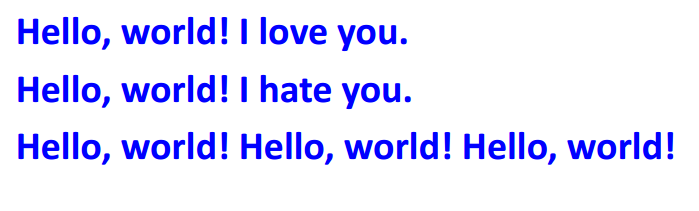
\includegraphics[width=0.5\textwidth]{diagrams/lz77_1.png}\end{figure}
\begin{figure}[H] \caption{Compression starts with literal representation.}
\centering
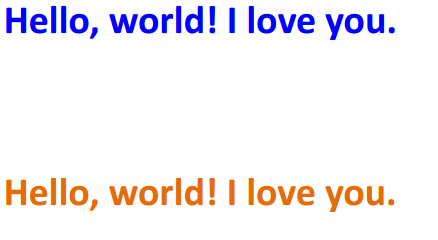
\includegraphics[width=0.35\textwidth]{diagrams/lz77_2.png}\end{figure}
\begin{figure}[H] \caption{We then use a pointer at distance 26 and length 16.}
\centering
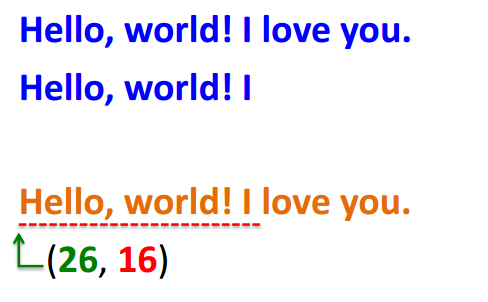
\includegraphics[width=0.35\textwidth]{diagrams/lz77_3.png}\end{figure}
\begin{figure}[H] \caption{We continue with literal.} \centering
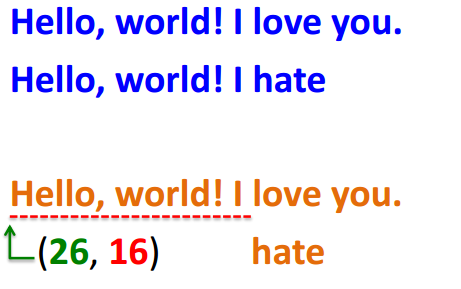
\includegraphics[width=0.35\textwidth]{diagrams/lz77_4.png}\end{figure}
\begin{figure}[H] \caption{We use a pointer pointing to a pointer.} \centering
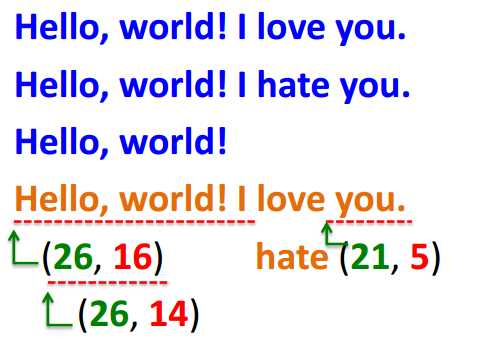
\includegraphics[width=0.35\textwidth]{diagrams/lz77_5.png}\end{figure}
\begin{figure}[H] \caption{We then use a pointer pointing to a pointer pointing
to a pointer.} \centering
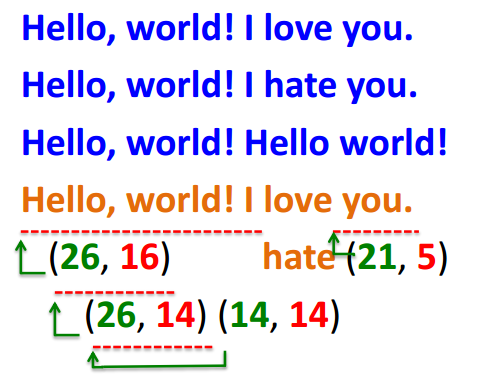
\includegraphics[width=0.35\textwidth]{diagrams/lz77_6.png}\end{figure}
\begin{figure}[H] \caption{Finally, we use a pointer pointing to itself.}
\centering
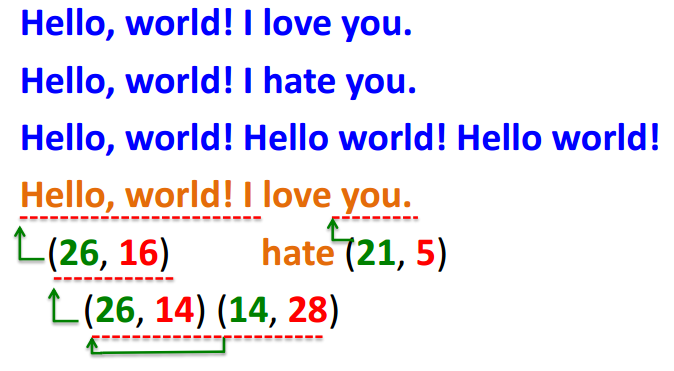
\includegraphics[width=0.5\textwidth]{diagrams/lz77_7.png}\end{figure}


\subsection{Huffman coding}

Huffman coding is also a lossless data compression algorithm developed by David
A. Huffman and published in 1952. \cite{huffman} When compressing a text, a
variable-length code table is created to map source symbols to bitstreams. Each
source symbol can be of less or more bits than originally and the mapping table
is used to translate source symbols into bitstreams during compression and vice
versa during decompression. The mapping table could be represented by a binary
tree of nodes. Each leaf node represents a source symbol, which can be accessed
from the root by following the left path for 0 and the right path for 1. Each
source symbol can be represented only by leaf nodes, therefore the code is
prefix-free, meaning no bitstream representing a source symbol can be the prefix
of any other bitstream representing a different source symbol. The final mapping
of source symbols to bistreams is calculated by finding the frequency of
appearance for each source symbol of the plaintext. That way, most common
symbols can be coded in shorter bitstreams, thus compressing the initial text.

Below follows an example of a plaintext and a valid Huffman tree for compressing
it:

\bigskip \centerline{\textit{\textbf{Chancellor on bring of second bailout for
banks}} \footnote{\url{https://en.bitcoin.it/wiki/Genesis_block}}}

\bigskip \centerline{\textbf{Frequency Analysis}}

\begin{table}[H] \centering \begin{tabular}{ | l | l | l | l | } \hline
\textbf{o}: 6 & \textbf{n}: 5 & \textbf{r}: 3 & \textbf{l}: 3 \\ \textbf{b}: 3 &
\textbf{c}: 3 & \textbf{a}: 3 & \textbf{s}: 2 \\ \textbf{k}: 2 & \textbf{e}: 2 &
\textbf{i}: 2 & \textbf{f}: 2 \\ \textbf{h}: 1 & \textbf{d}: 1 & \textbf{t}: 1 &
\textbf{u}: 1 \\ \hline \end{tabular} \end{table}

\centerline{\textbf{Huffman tree}}

\begin{table}[H] \centering \begin{tabular}{ | l | l | l | l | } \hline
\textbf{o}: 00 & \textbf{n}: 01 & \textbf{r}: 1000 & \textbf{l}: 1001 \\
\textbf{b}: 1010 & \textbf{c}: 1011 & \textbf{a}: 11000 & \textbf{s}: 11001 \\
\textbf{k}: 11010 & \textbf{e}: 11011 & \textbf{i}: 11100 & \textbf{f}: 1111000
\\ \textbf{h}: 1111001 & \textbf{d}: 1111010 & \textbf{t}: 1111011 & \textbf{u}:
1111100 \\ \hline \end{tabular} \end{table}

\centerline{\textbf{Initial text size: 320 bits}} \centerline{\textbf{Compressed
text size: 167 bits}}

\section{Same-origin policy}\label{sec:sameorigin}

Same-origin policy is an important aspect of the web application security model.
According to that policy, a web browser allow scripts contained in one page to
access data in a second page only if both pages have the same \textit{origin}.
Origin is defined as the combination of Uniform Resource Identifier scheme,
hostname and port number. For example, a document retrieved from the website
\textit{http://example.com/target.html} is not allowed under the same-origin
policy to access the Document-Object Model of a document retrieved from
\textit{https://head.example.com/target.html}, since the two websites have
different URI schema (\textit{http} vs \textit{https}) and different hostname
(\textit{example.com} vs \textit{head.example.com}).

Same-origin policy is particularly important in modern web applications, that
rely greatly on HTTP cookies to maintain authenticated sessions. If same-origin
policy was not implemented the data confidentiality and integrity of cookies, as
well as every other content of web pages, would have been compromised. However,
despite the application of same-origin policy by modern browsers, there exist
attacks that enable an adversary to bypass it and breach a user's communication
with a website. Two such major types of vulnerabilities, cross-site scripting
and cross-site request forgery are described in the following subsections.

\subsection{Cross-site scripting}

Cross-site scripting (XSS) is a security vulnerability that allows an adversary
to inject client-side script into web pages viewed by other users. That way,
same-origin policy can be bypassed and sensitive data handled by the vulnerable
website may be compromised. XSS could be divided into two major types,
\textit{non-persistent} and \textit{persistent}
\footnote{\url{https://en.wikipedia.org/wiki/Cross-site_scripting}}, which we
will describe below.

Non-persistent XSS vulnerabilities are the most common. They show up when the
web server does not parse the input in order to escape or reject HTML control
characters, allowing for scripts injected to the input to run unnoticeable.
Usual methods of performing non-persistent XSS include mail or website url links
and search requests.

Persistent XSS occurs when data provided by the attacker are stored by the
server. Responses from the server to different users will then include the
script injected from the attacker, allowing it to run automatically on the
victim's browsers without needing to target them individually. An example of
such attack is when posting texts on social networks or message boards.

\subsection{Cross-site request forgery}

Cross-site request forgery (CSRF) is an exploit that allows an attacker to issue
unauthorized commands to a website, on behalf of a user the website trusts.
Hence the attacker can forge a request to perform actions or post data on a
website the victim is logged in, execute remote code with root privileges or
compromise a root certificate, resulting in a breach of a whole public key
infrastructure (PKI).

CSRF can be performed when the victim is trusted by a website and the attacker
can trick the victim's browser into sending HTTP requests to that website. For
example, when a Alice visits a web page that contains the HTML image tag
\textit{<img
src="\url{http://bank.example.com/withdraw?account=Alice&amount=1000000&for=Mallory}">}
\footnote{\url{https://en.wikipedia.org/wiki/Cross-site_request_forgery}} that
Mallory has injected, a request from Alice's browser to the example bank's
website will be issued, stating for an amount of 1000000 to be transfered from
Alice's account to Mallory's. If Alice is logged in the example bank's website,
the browser will include the cookie containing Alice's authentication
information in the request, making it a valid request for a transfer. If the
website does not perform more sanity checks or further validation from Alice,
the unauthorized transaction will be completed. An attack such as this is very
common on Internet forums that allow users to post images.

A method of mitigation of CSRF is a Cookie-to-Header token. The web application
sets a cookie that contains a random token that validates a specific user
session. Javascript on client side reads that token and includes it in a HTTP
header sent with each request to the web application. Since only Javascript
running within the same origin will be allowed to read the token, we can assume
that it's value is safe from unauthorized scripts to read and copy it to a
custom header in order to mark a rogue request as valid.

\section{Transport Layer Security}\label{sec:tls}

Transport Layer Security (TLS) is a protocol that provides communications
security over the internet, allowing a server and a client to communicate in a
way that prevents eavesdropping, tampering or message forgery. \cite{tls12}

The users negotiate a symmetric key via assymetric cryptography that is provided
by X.509 certificates, therefore there exist certificate authorities and a
public key infrastructure (PKI), in order for the certificates to be verified
for their owners. However, it can be understood that, due to their key role,
certificate authorities are points of failure in the system, enabling for
Man-in-the-Middle attacks, in a case when an adversary has managed to forge
a root certificate.

Apart from certificate-related attacks, a well-known category is compression
attacks. \footnote{\url{https://tools.ietf.org/html/rfc7457}} Such attacks
exploit TLS-level compression so as to decrypt ciphertext. In this document, we
investigate the threat model and performance of such an attack,
\href{http://breachattack.com}{BREACH}.

In the following subsections we will briefly describe some of the protocol
details, especially handshake and the format of TLS records.

\subsection{TLS handshake}

\begin{figure}[H] \caption{TLS handshake flow.} \centering
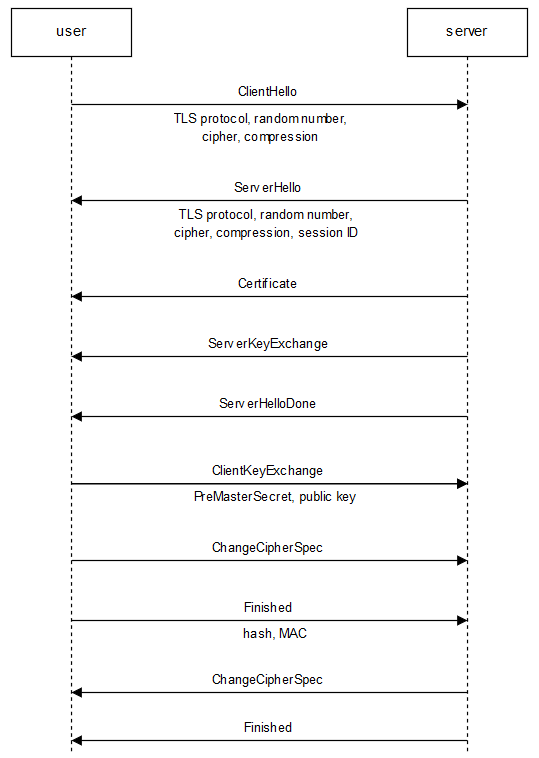
\includegraphics[width=0.7\textwidth]{diagrams/tls_handshake.png}\end{figure}

This sequence diagram presents the functionality of TLS handshake. User and
server exchange the basic parameters of the connection, specifically the
protocol version, cipher suite, compression method and random numbers, with the
ClientHello and ServerHello records. The server then provides all information
needed from the user to validate and use the asymmetric server key, in order to
compute the symmetric key to be used in the rest of the communication. The
client computes a \textit{PreMasterKey}, that is sent to the server, which is
used by both parties to compute the symmetric key. Finally, both sides exchange
and validate hash and MAC over the previous messages, after which they both have
the ability to communicate safely.

The above flow describes the basic TLS handshake. Client-authenticated and
resumed handshakes have similar functionality, which are not relevant for the
purpose of this paper.

\subsection{TLS record}

\begin{figure}[H] \caption{TLS record.} \centering
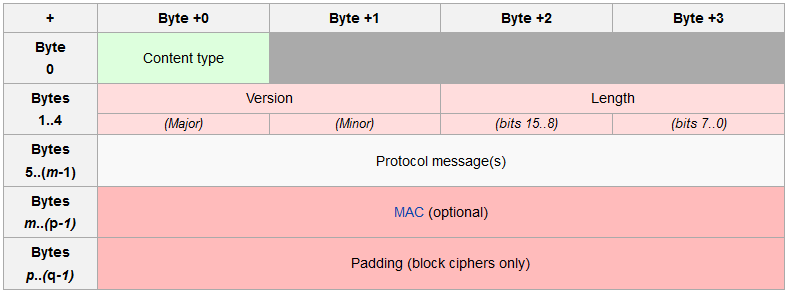
\includegraphics[width=1\textwidth]{diagrams/tls_record.png}\end{figure}

The above figure
\footnote{\url{https://en.wikipedia.org/wiki/Transport_Layer_Security}} depicts
the general format of all TLS records.

The first field describes the Record Layer Protocol Type contained in the
record, which can be one of the following:

\begin{table}[H] \centering \begin{tabular}{ | l | l | } \hline \textbf{Hex} &
\textbf{Type} \\ \hline 0x14 & ChangeCipherSpec \\ 0x15 & Alert \\ 0x16 &
Handshake \\ 0x17 & Appliation \\ 0x18 & Heartbeat \\ \hline \end{tabular}
\end{table}

The second field defines the TLS version for the record message, which is
identified my the major and minor version as below:

\begin{table}[H] \centering \begin{tabular}{ | l | l | l | } \hline
\textbf{Major} & \textbf{Minor} & \textbf{Version} \\ \hline 3 & 0 & SSL 3.0 \\
3 & 1 & TLS 1.0 \\ 3 & 2 & TLS 1.1 \\ 3 & 3 & TLS 1.2 \\ \hline \end{tabular}
\end{table}

The length of the contained record message, MAC and padding is then calculated
by the following two fiels as: \begin{math}256*(bits 15..8) + (bits
7..0)\end{math}.

Finally, the payload of the record, which, depending on the type, may be
encrypted, the MAC, if provided, and the padding, if needed, make up the rest of
the TLS record.

\section{Man-in-the-Middle}\label{sec:mitm}

Man-in-the-Middle (MitM) is one of the most common attack vectors, where an
attacker reroutes the communication of two parties, in order to be controlled
and possibly altered. The aggressiveness of the attack can vary from passive
eavesdropping to full control of the communication, as long as the attacker is
able to impersonate both parties and convince them to be trusted.

\begin{figure}[H] \caption{Man-in-the-Middle.} \centering
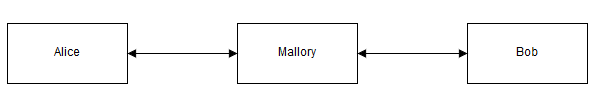
\includegraphics[width=1\textwidth]{diagrams/mitm.png}\end{figure}

MitM attacks can be mitigated by using end-to-end cryptography, mutual
authentication or PKIs. However, some attacks manage to bypass such mitigation
techniques. Below, we descripe two such attacks, ARP Spoofing and DNS cache
poisoning.

\subsection{ARP Spoofing} ARP spoofing

\footnote{\url{https://en.wikipedia.org/wiki/ARP_spoofing}} is a technique where
an attacker sends Address Resolution Protocol (ARP) messages over the network,
so as to assosiate the MAC address with the IP address of another host. That
way, the attacker may intercept the traffic of the network, modify or deny
packets, performing denial of service, MitM or session hijacking attacks.

\begin{figure}[H] \caption{Arp Spoofing.} \centering
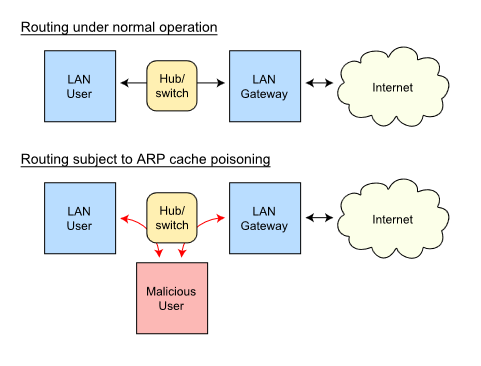
\includegraphics[width=0.8\textwidth]{diagrams/arp_spoofing.png}\end{figure}

ARP spoofing can be also used for legitimate reasons, when a developer needs to
debug IP traffic between two hosts. That way, the developer can act as proxy
between the two hosts or configure the switch that is normally used by the two
parties to forward traffic for monitoring.

\subsection{DNS spoofing}

\begin{figure}[H] \caption{DNS Spoofing.} \centering
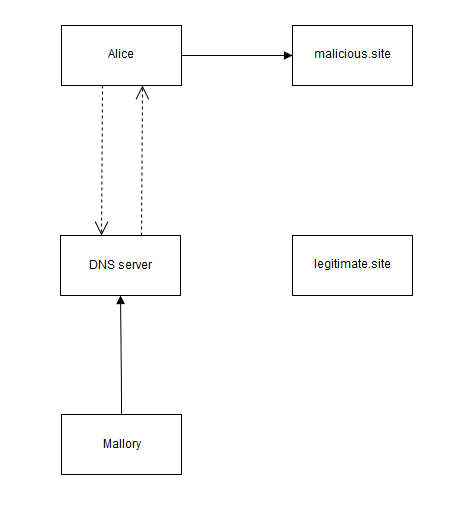
\includegraphics[width=0.5\textwidth]{diagrams/dns_spoofing.png}\end{figure}

DNS spoofing (or DNS cache poisoning) is an attack, when the adversary
introduces data into a Domain Name System resolver's cache, in order to return
an incorrect address for a specific host.

DNS servers are usually provided by Internet Service Providers (ISPs), used to
resolve IP addresses to human-readable hostnames faster. A malicious employee,
or anyone that has gained unauthorized access to the server, can then perform
DNS poisoning, affecting every user that is being serviced by that server.

\chapter{Partially Chosen Plaintext Attack}\label{ch:pcpa}

Traditionally, cryptographers have used games for security analysis. Such games
include the indistinguishability under chosen-plaintext-attack (IND-CPA), the
indistinguishability under chosen ciphertext attack/adaptive chosen ciphertext
attack (IND-CCA1, IND-CCA2) etc
\footnote{\url{https://en.wikipedia.org/wiki/Ciphertext_indistinguishability}}.
In this chapter, we introduce a definition for a new property of encryption
schemes, called indistinguishability under partially-chosen-plaintext-attack
(IND-PCPA). We will also show provide comparison between IND-PCPA and other
kwown forms of cryptosystem properties.

\section{Partially Chosen Plaintext Indistinguishability}\label{sec:indpcpa}

\subsection{Definition} IND-PCPA uses a definition similar to that of IND-CPA.
For a probabilistic asymmetric key encryption algorithm, indistinguishability
under partially chosen plaintext attack (IND-PCPA) is defined by the following
game between an adversary and a challenger.

\begin{itemize} \item The challenger generates a pair \begin{math}P_k,
S_k\end{math} and publishes \begin{math}P_k\end{math} to the adversary.  \item
The adversary may perform a polynomially bounded number of encryptions or other
operations.  \item Eventually, the adversary submits two distinct chosen
plaintexts \begin{math}M_0, M_1\end{math} to the challenger.  \item The
challenger selects a bit \begin{math}b\in{0, 1}\end{math} uniformly at random.
\item The adversary can then submit any number of selected plaintexts
\begin{math}R_i, i\in N, |R| \geq 0\end{math}, so the challenger sends the
ciphertext \begin{math}C_i = E(P_k, M_b||R_i)\end{math} back to the adversary.
\item The adversary is free to perform any number of additional computations or
encryptions, before finally guessing the value of \begin{math}b\end{math}.
\end{itemize}

A cryptosystem is indistinguishable under partially chosen plaintext attack, if
every probabilistic polynomial time adversary has only a negligible advantage on
finding \begin{math}b\end{math} over random guessing. An adversary is said to
have a negligible advantage if it wins the above game with probability
\begin{math}\frac{1}{2} + \epsilon(k)\end{math}, where
\begin{math}\epsilon(k)\end{math} is a negligible function in the security
parameter \begin{math}k\end{math}.

Intuitively, we can think that the adversary has the ability to modify the
plaintext of a message, by appending a portion of data of his own choice to it,
without knowledge of the plaintext itself. He can then acquire the ciphertext of
the modified text and perform any kinds of computations on it. A system could
then be described as IND-PCPA, if the adversary is unable to gain more
information about the plaintext, than he could by guessing at random.

\subsection{IND-PCPA vs IND-CPA}

Suppose the adversary submits the empty string as the chosen plaintext, a choice
which is allowed by the definition of the game. The challenger would then send
back the ciphertext \begin{math}C_i = E(P_k, M_b||"\ ") = E(P_k, M_b)\end{math},
which is the ciphertext returned from the challenger during the IND-CPA game.
Therefore, if the adversary has the ability to beat the game of IND-PCPA, i.e. if
the system is not indistinguishable under partially chosen plaintext attacks, he
also has the ability to beat the game of IND-CPA. Thus we have shown that
IND-PCPA is at least as strong as IND-CPA.

\section{PCPA on compressed encrypted protocols}\label{sec:cepcpa}

\subsection{Compression-before-encryption and vice versa} When having a system
that applies both compression and encryption on a given plaintext, it would be
interesting to investigate the order the transformations should be executed.

Lossless data compression algorithms rely on statistical patters to reduce the
size of the data to be compressed, without losing information. Such a method is
possible, since most real-world data has statistical redundancy. However, it can
be understood from the above that such compression algorithms will fail to
compress some data sets, if there is no statistical pattern to exploit.

Encryption algorithms rely on adding entropy on the ciphertext produced. If the
ciphertext contains repeated portions or statistical patterns, such behaviour
can be exploited to deduce the plaintext.

In the case that we apply compression after encryption, the text to be
compressed should demostrate no statistical analysis exploits, as described
above. That way compression will be unable to reduce the size of the data. In
addition, compression after encryption does not increase the security of the
protocol.

On the other hand, applying encryption after compression seems a better
solution. The compression algorithm can exploit the statistical redundancies of
the plaintext, while the encryption algorithm, if applied perfectly on the
compressed text, should produce a random stream of data. Also, since compression
also adds entropy, this scheme should make it harder for attackers who rely on
differential cryptanalysis to break the system.

\subsection{PCPA scenario on compression-before-encryption protocol}

Let's assume a system that composes encryption and compression in the following
manner:

\begin{math}c = Encrypt(Compress(m))\end{math}

where \begin{math}c\end{math} is the ciphertext and \begin{math}m\end{math} is
the plaintext.

Suppose the plaintext contains a specific secret, among random strings of data,
and the attacker can issue a PCPA with a chosen plaintext, which we will call
reflection. The plaintext then takes the form:

\begin{math}m = n_1 || secret || n_2 || reflection || n_3\end{math}

where \begin{math}n_1, n_2, n_3\end{math} are random nonces.

If the reflection is equal to the secret, the compression mechanism will
recognize the pattern and compress the two portions. In other case, the two
strings will not demonstrate any statistical redundancy and compression will
perform worse. As a result, in the first case the data to be encrypted will be
smaller than in the second case.

Most commonly encryption is done by a stream or a block cipher. In the first
case, the lengths of a plaintext and the corresponding ciphertext are identical,
whereas in the second case they differ by the number of the padding bits, which
is relatively small. That way, in the above case, an adversary could identify a
pattern and extract information about the plaintext, based on the lengths of the
two ciphertexts.

\backmatter
\cleardoublepage % start at the next odd page
\phantomsection % correct hyperlinking
\bibliography{references}
\bibliographystyle{ieeetr}
%\include{glossary}

\end{document}
